\documentclass{scrartcl}
\usepackage{amsmath,amssymb,graphicx,wrapfig,ulem,qtree}
\setkomafont{disposition}{\normalfont\bfseries}

\title{Foundations of Computer Science}
\subtitle{Notes from 02-26-2015}
\author{Kenny Roffo}

\begin{document}

\maketitle
\tableofcontents\pagebreak

\section{Formal Languages}

\subsection{Definitions}

\begin{enumerate}

\item A \underline{symbol} is the basic indivisible entity

Natural Languages: words, not letters

\item An \underline{alphabet} is a finite, nonempty set of symbols

$\Sigma$ is typically used as the name for the alphabet

Natural languages: $\Sigma=\{$\emph{all words in English}$\}$ - Lexicon 

\item A \underline{string} (over $\Sigma$) is a finite sequence of symbols (over $\Sigma$)

  Properties: \begin{itemize}
  \item \underline{length}
  \item \underline{empty string} denoted $\lambda$
  \item \underline{concatenation}
  \item $\lambda$ identity of concatenation
  \end{itemize} 

\item $\Sigma ^*$ is the set of all finite strings over $\Sigma$

e.q. $\Sigma=\{0,1\}$, $\Sigma ^* = \{$all strings of $0$ and $1\}$

$\Sigma$ is an alphabet\\
$\Sigma ^*$ is defined recursively

$\lambda$ is an element of $\Sigma ^*$, and if $w \in \Sigma ^*, a \in \Sigma$, then $wa \in \Sigma ^*$

\item A \underline{language} $L$ is any set of strings formed from a given alphabet $\Sigma$\\
$\phi$ is a language over \emph{any} alphabet\\
$\Sigma$ is a language over $\Sigma$\\
$\Sigma ^*$ is a language over $\Sigma$
\end{enumerate}

\subsection{Examples}

\begin{enumerate}

\item $\Sigma = \{b\}$\\
$\Sigma^*=\{\lambda, b, bb, bbb, ...\}$

\item $\Sigma = \{a,b\}$\\
$\Sigma^*=\{\lambda, a, b, aa, ab, ba, bb, ...\}$\\
L is a language over $\Sigma$ that is defined recursively:
ex: $L=\{w|w=a^nb^n, n\ge1\}$\\
($a^n$ means $aaa...a$ n times)\\
Thus $L=\{ab, aabb, aaabbb, aaaabbbb, ...\}$, if $w \in L$, then $awb \in L$\pagebreak

\item Let $L_n={a^nb^n}$. Then $L = L_0 \cup L_1 \cup L_2 \cup ... $

\item Let $\Sigma_i$ be the language of $i$ length strings in the alphabet $\Sigma=\{a,b\}$.\\
Then $\Sigma_0=\{\lambda\}$, $\Sigma_1=\{a,b\}$, $\Sigma_2=\{aa, ab, ba, bb\}$, ...\\
It follows that the language $\Sigma^*=\Sigma_0 \cup \Sigma_1 \cup \Sigma_2 \cup ...=\bigcup_{i=1}^{\infty} \Sigma_i$

\end{enumerate}

\subsection{What is $\Sigma^*$}

Concatenation - Making new strings from existing strings. We can also concatenate strings with languages and languages with languages.
If $L_1$ and $L_2$ are languages, then $L_1L_2=\{w_1w_2|w_1 \in L_1, w_2 \in L_2\}$\\

ex: Let $L_1=\{$in,out$\}$ and $L_2=\{$law,door,ward$\}$.

Then $L_1L_2=\{$inlaw,outlaw,indoor,outdoor,inward,outward$\}$\\\\
$\Sigma^*$ is the set of all strings made from the alphabet $\Sigma$. But why $\Sigma^*$?\\
$\Sigma^*$ is the result of concatenating $\Sigma$ with itself zero or more times.\\
$\Sigma^+$ is the result of concatenating $\Sigma$ with itself one or more times.

This is called the positive closure of $\Sigma$.\\\\

\section{Regular Expressions}

\subsection{What is a Regular Expression?}

A \emph{regular expression} (regex) is a way to specify patterns for strings using union (or), concatenation, and $^*$\\\\
A regex over $\Sigma$ is defined:

\emph{Basis}: Every $a \in \Sigma$ is a regex over $\Sigma$

\emph{Recursive}: If $u$ and $v$ are regex over $\Sigma$ then $u|v$, $uv$, and $u^*$ are all regex over $\Sigma$\\\\
Here, $|$ means \emph{or} and $^*$ means 0 or more. When in doubt, use parentheses.\\\\
grep - general regular expression parser - a Unix command which searches a file for a pattern defined by a regex.

\pagebreak
Let $X=\{a,ab,aba\}$ and $Y=\{b,bb\}$. Then
\begin{itemize}
\item $XY=\{ab,abb,abb,abbb,abab,ababb\}$ (Concatenation)
\item $X|Y=\{a,ab,aba,b,bb\}$ (Like union)
\item $X^*=\{a,aa,aaa,...,aab,ab,abab,ababab,...,aab,aaba,aaab,ababa,...\}$ 

(All possible strings from 0 or more concatenations)
\item $ababa \in X^*$
\item $ababa \in XY^*$
\item $ab(ab)^*a$ is a regex that matches $ababa$
\end{itemize}

\section{Finite State Machines}
\subsection{The Vending Machine}
Consider a vending machine which contains Jelly beans and Gum. The Machine has inputs
\begin{itemize}
\item N - 5 cents
\item D - 10 cents
\item J - Jelly Bean (Costs 20 cents)
\item G - Gum (Costs 15 cents)
\end{itemize}
These can be represented by $\Sigma=\{N,D,J,G\}$. The machine also has outputs
\begin{itemize}
\item b - beep when money is added
\item j - jelly bean dispensed
\item g - gum dispensed
\end{itemize}
Design a \underline{Finite State} machine - a machine with a finite number of ``things to remember''
This vending machine has to ``remember'':
\begin{itemize}
\item total money deposited (but not he order in which coins are desposited)
\item which product is selected
\end{itemize}
States are drawn with circles and named on the inside:\\

\begin{wrapfigure}[15]{r}[12pt]{3in}
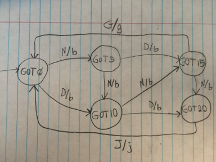
\includegraphics{./VMStateDiagram.png}\\
\end{wrapfigure}

For our Vending Machine the states are described by how much money is in the machine, and the transitions represent money input, or a purchase or gum or a jelly bean. The states live in the set $Q=\{GOT\emptyset,GOT5,GOT10,GOT15,GOT20\}$.\\ State transitions are defined by a function $\delta: Q\times\Sigma\rightarrow Q$. As an example, 
\begin{displaymath}
(GOT5)(N) \rightarrow GOT10 
\end{displaymath}

Here is an example of a state transition diagram.

\subsection{Finite State machine}
A finite state machine has one or more states. For the vending machine in the previous section the inital and final states happen to be the same. Any \underline{path} in the state transition diagram is called a \underline{computation}. Any path in a finite state machine which starts in the initial state and ends in the final state is called an \emph{acceptable} path.\\

A finite state machine must have:
\begin{itemize}
\item An input mechanism
\item A computing mechanism
\item An output mechanism
\end{itemize}

We use ordered pairs to reference what has happened in the fsm. Referring back to the vending machine, here is an example:\\\\
$(GOT5,NNNDG)\rightarrow(GOT10,NNDG)\rightarrow(GOT15,NDG)\rightarrow(GOT20,DG)\rightarrow$\\
$(GOT20,G)\rightarrow(GOT\emptyset,\lambda)$\\

The first part of the pair represents the current state while the second represents the input. Each pair is called an \emph{instantaneous configuration}.

A finite state machine is defined by a 5-tuple: $M=(Q,\Sigma,\delta,q_0,F)$:
\begin{itemize}
\item $Q$: finite, nonempty set of states
\item $\Sigma$: alphabet (finite, nonempty set of symbols)
\item $\delta$: $Q\times\Sigma\rightarrow Q$ is the state transition function
\item $q_0$: initial state
\item $F\subset Q$ : set of final states
\end{itemize}

\subsection{The Turing Machine}

Alan Turing was one of the most influential scientists of the $20^{th}$ century. One of his contributions was the idea of a Turing Machine.\\

A Turing Machine is a machine that can solve any computable problem. In other words, if a problem is able to be computed, a Turing Machine can solve that problem.\\

The Wikipedia definition of a Turing machine:

 \emph{A \textbf{Turing machine} is a hypothetical device that manipulates symbols on a strip of tape according to a table of rules. Despite its simplicity, a Turing machine can be adapted to simulate the logic of any computer algorithm, and is particularly useful in explaining the functions of a CPU inside a computer.}\\\\
\textbf{The Man, the Wolf, the Goat and the Cabbage}\\\\
Consider this classic problem:\\

A man once had to travel with a wolf, a goat and a cabbage. He had to take good care of them, since the wolf would like to taste a.piece of goat if he would get the chance, while the goat appeared to long for a tasty cabbage. After some traveling, he suddenly stood before a river. This river could only be crossed using the small boat laying nearby at a shore. The boat was only good enough to take himself and one of his loads across the river. The other two subjects/objects he had to leave on their own. How must the man row across the river back and forth, to take himself as well as his luggage safe to the other side of the river, without having one eating another? \\

A table can be constructed similar to show the possible different states. States that are not allowed are crossed out. The route I chose to take is in bold, and the next possible states from there are listed on the next line. Note that there are infinitely many solutions. I chose my solution as it seemed the most logical to me on the fly.

\begin{center}
\begin{tabular} { |c|c c c c| }
\hline
&M&W&G&C\\
\hline
MWGC-&WGC-M&\sout{GC-MW}&\textbf{WC-MG}&\sout{WG-MC}\\
WC-MG&\textbf{MWC-G}&X&MWGC-&X\\
MWC-G&WC-MG&C-MWG&X&\textbf{W-MGC}\\
W-MGC&\sout{MW-GC}&X&\textbf{MWG-C}&MWC-G\\
MWG-C&\sout{WG-MC}&\textbf{G-MWC}&W-MGC&X\\
G-MWC&\textbf{MG-WC}&MWG-C&X&MGC-W\\
MG-WC&G-MWC&X&\textbf{-MWGC}&X\\
\hline
\end{tabular}
\end{center}\pagebreak

\subsection{Non-deterministic Finite State Machines}
Let $\Sigma=\{a,b\}$. Design a finite state machine that accepts all strings over $\Sigma$ that contain the substring $bab$:\\

Regular Expression: $(a|b)^*bab(a|b)^*$
\begin{center}
\begin{tabular} {|c|c c|}
\hline
$\delta$&$a$&$b$\\
\hline
$q_0$&$q_0$&$q_0,q_1$\\
$q_1$&$q_2$&...\\
$q_2$&...&$q_3$\\
$q_3$&$q_3$&$q_3$\\
\hline
\end{tabular}
\end{center}

As seen in the table, if the state is $q_0$ and the input is $a$, then the machine has two options. We call this non-deterministic, and thus we call the machine a \emph{non-deterministic finite state machine}. Let $M$ be a non-deterministic finite state machine: Then $$M=(Q,\Sigma,q,\delta,F)$$ where $$\delta : Q \times \Sigma \rightarrow \rho(Q)$$ Recall that $\rho(S)$ is the power set of $S$. An alternate way of making the table above would be:

\begin{center}
\begin{tabular} {|c|c c|}
\hline
$\delta$&$a$&$b$\\
\hline
$q_0$&$\{q_0\}$&$\{q_0,q_1\}$\\
$q_1$&$\{q_2\}$&$\emptyset$\\
$q_2$&$\emptyset$&$\{q_3\}$\\
$q_3$&$\{q_3\}$&$\{q_3\}$\\
\hline
\end{tabular}
\end{center}

We define a new function, $\delta' : \rho(q)\times\Sigma\rightarrow\rho(Q)$

\begin{center}
\begin{tabular} {|c|c c|}
\hline
$\delta_1$&$a$&$b$\\
\hline
$\{q_0\}$&$\{q_0\}$&$\{q_0,q_1\}$\\
$\{q_0,q_1\}$&$\{q_0,q_2\}$&$\{q_0,q_1\}$\\
$\{q_0,q_2\}$&$\{q_0\}$&$\{q_0,q_1,q_3\}$\\
$\{q_0,q_1,q_3\}$&$\{q_0,q_2,q_3\}$&$\{q_0,q_1,q_3\}$\\
$\{q_0,q_2,q_3\}$&$\{q_0,q_3\}$&$\{q_0,q_1,q_3\}$\\
$\{q_0,q_3\}$&$\{q_0,q_3\}$&$\{q_0,q_1,q_3\}$\\
\hline
\end{tabular}
\end{center}

The sets on the left are determined as the table is constructed based on what appears on the right. Now we let
\begin{align*}
\{q_0\} &= 0\\
\{q_0,q_1\} &= 01\\
\{q_0,q_2\} &= 02\\
\{q_0,q_1,q_3\} &= 013\\
\{q_0,q_2,q_3\} &= 023\\
\{q_0,q_3\} &= 03\\
\end{align*}
Then our machine becomes $M'(Q',\Sigma,\delta',0,F)$ with
\begin{align*}
Q'&=\{0,01,02,013,023,03\}\\
\Sigma&=\{a,b\}\\
\delta' &: \rho(Q)\times\Sigma\rightarrow \rho(Q)\\
F&=\{013,023,03\}
\end{align*}

\begin{center}
\begin{tabular} {|c|c c|}
\hline
$\delta'$&$a$&$b$\\
\hline
0& 0 & 01\\
01& 02 & 01\\
02& 0 & 013 \\
013& 023 & 013\\
023 & 03 & 013\\
03 & 03 & 013\\
\hline
\end{tabular}
\end{center}
This may feel a little uneasy at first, but we now have a deterministic finite state machine (DFA).\pagebreak

\subsection{Minimizing a DFA}
We have a method for ensuring our DFA is minimal. Let's show this by an example. Consider the DFA from the end of the previous subsection:\\
\begin{center}
\begin{tabular} {|c|c c|}
\hline
$\delta'$&$a$&$b$\\
\hline
0& 0 & 01\\
01& 02 & 01\\
02& 0 & 013 \\
013& 023 & 013\\
023 & 03 & 013\\
03 & 03 & 013\\
\hline
\end{tabular}
\end{center}\ \\
This DFA is not minimal, so we start by making a partition of the states. One set will be the final states, and the other set will be the rest of the states:
$$\Pi_0:\ ^A[0\ 01\ 02]\ ^B[013\ 023\ 03]$$
From here we look at which sets each element maps to. For example, when the inputs are $a$ and $b$, the outputs are elements of the sets $A$ and $A$ for 0, $A$ and $A$ for 01, $A$ and $B$ for 02, etc. Since 0 and 01 map to the same sets for both inputs, they will stay together. However, 02 will branch off into its own set, called a singleton. Note that if elements of $A$ have the same mappings as elements of $B$ they do not become members of the same set at the next level of the process since they came from different sets. This means the next step gives:
$$\Pi_1:\ ^C[0\ 01]\ ^D[02]\ ^E[013\ 023\ 03]$$
We now execute the process again to have:
$$\Pi_2:\ ^F[0]\ ^G[01]\ ^H[02]\ ^I[013\ 023\ 03]$$
Finally, we will do this one last time to see that $\Pi_3=\Pi_2$, and thus the process no longer reduces the partition:
$$\Pi_3:\ ^F[0]\ ^G[01]\ ^H[02]\ ^I[013\ 023\ 03]$$
Now we define:
\begin{align*}
0&=F\\
01&=G\\
02&=H\\
0123&=I
\end{align*}
And define our minimal finite state machine:
\begin{center}
\begin{tabular} {|c|c c|}
\hline
$\delta$&$a$&$b$\\
\hline
0& 0 & 01\\
01& 02 & 01\\
02& 0 & 0123 \\
0123& 0123 & 0123\\
\hline
\end{tabular}
\end{center}\ \\

%We want to turn this in to a deterministic finite state machine. Let's keep track of all possible moves of our machine on the string $ababa$% using a tree:
%\Tree
%    [q_0 
%        [q_0
%            [q_0
%                [q_0
%                    [q_0 q_0]
%                    [q_1 q_2]
%                ] 
%            ]
%            [q_1
%                [q_2 [q_3 [q_3]]]
%            ] 
%        ]
%    ]
%
\subsection{Converting NFA to DFA with $\epsilon$ moves}

To convert an NFA to a DFA we will compute the $\epsilon$-closure of every state.\\

$\epsilon$-moves are moves without any input.

$\epsilon-c(q) \equiv \{s|s \text{ can be reached from } q \text{ by an $\epsilon$-move}\}$\\

Consider the NFA with $\epsilon$-moves:
\begin{center}
\begin{tabular} {|c|c c c|}
\hline
$\delta$&0&1&$\epsilon$\\
\hline
$q_0$ & $\emptyset$ & $\emptyset$ & $\{e0,e1\}$\\
$e0$ & $\{o0\}$ & $\{e0\}$ & $\emptyset$\\
$e1$ & $\{e1\}$ & $\{o1\}$ & $\emptyset$\\
$o0$ & $\{e0\}$ & $\{o0\}$ & $\emptyset$\\
$o1$ & $\{o1\}$ & $\{e1\}$ & $\emptyset$\\
\hline
\end{tabular}
\end{center}

We will find the $\epsilon$-closure of every state:
\begin{align*}
\epsilon-c(q_0) &= \{q_0,e0,e1\}\\
\epsilon-c(e0) &= \{e0\}\\
\epsilon-c(e1) &= \{e1\}\\
\epsilon-c(o0) &= \{o0\}\\
\epsilon-c(o1) &= \{o1\}\\
\end{align*}

Now we construct $\delta'$ with NFA$\rightarrow$ DFA except add $\epsilon$-closures of all resulting states.

\begin{center}
\begin{tabular} {|c|c c|}
\hline
$\delta'$&$0$&$1$\\
\hline
$\{q_0,e0,e1\}$ & $\{o0,e1\}$ & $\{e0,o1\}$\\
$\{o0,e1\}$ & $\{e0,e1\}$ & $\{o0,o1\}$\\
$\{e0,o1\}$ & $\{o0,o1\}$ & $\{e0,e1\}$\\
$\{e0,e1\}$ & $\{o0,e1\}$ & $\{e0,o1\}$\\
$\{o0,o1\}$ & $\{e0,01\}$ & $\{o0,e1\}$\\
\hline
\end{tabular}
\end{center}
Now we define:
\begin{align*}
\{q_0,e_1,e_0\} &= i\\
\{o0,e1\} &= o0e1\\
\{e0,o1\} &= e0o1 \text{  and so on...}\\
\end{align*}\ \\\ \\

The DFA is now

\begin{center}
\begin{tabular} {|c|c c|}
\hline
$\delta'$&$0$&$1$\\
\hline
$i$ & $o0e1$ & $e0o1$\\
$o0e1$ & $e0e1$ & $o0o1$\\
$e0o1$ & $o0o1$ & $e0e1$\\
$e0e1$ & $o0e1$ & $e0o1$\\
$o0o1$ & $e001$ & $o0e1$\\
\hline
\end{tabular}
\end{center}

\section{Sequential Machines}
Sequential machines have outputs, like our vending machine.\\
State transition: $\delta(p,a)=q$ \ \ $\delta : Q \times \Sigma \rightarrow Q$\\
$\Sigma$ is an input alphabet\\
$\epsilon(p,a)=o$, $p$ is the state, $a$ is the input symbol, $o$ is the output symbol\\

\underline{Sequential Machine}:
\begin{itemize}
\item $Q$: Set of states
\item $\Sigma$: input alphabet
\item $\Delta$: output alphabet
\item $\delta:\ Q\times\Sigma\rightarrow Q$: state transition function
\item $\epsilon: Q\times\Sigma\rightarrow\Delta$: output function
\item $q_0$: initial state
\end{itemize}\ \\
\textbf{Ex}:\\\\
$M=(Q,\Sigma,\Delta,\delta,\epsilon,q_0)$\\
$Q=\{A,B,C,D,E,F\}$\\
$\Sigma=\{0,1\}$\\
$\delta:\ Q\times\Sigma\rightarrow Q$\\
$q_0=A$\\
$\Delta=\{0,1\}$\\
$\epsilon:\ Q\times\Sigma\rightarrow\Delta$\\\\
\begin{minipage}{0.45\linewidth}\centering
\begin{tabular} {|c|c c|}
\hline
$\delta$&$0$&$1$\\
\hline
$A$ & $E$ & $D$\\
$B$ & $F$ & $D$\\
$C$ & $E$ & $B$\\
$D$ & $F$ & $B$\\
$E$ & $C$ & $F$\\
$F$ & $B$ & $C$\\
\hline
\end{tabular}
\end{minipage}
\begin{minipage}{0.45\linewidth}\centering
\begin{tabular} {|c|c c|}
\hline
$\epsilon$&$0$&$1$\\
\hline
$A$ & $0$ & $1$\\
$B$ & $0$ & $0$\\
$C$ & $0$ & $1$\\
$D$ & $0$ & $0$\\
$E$ & $0$ & $1$\\
$F$ & $0$ & $0$\\
\hline
\end{tabular}
\end{minipage}\\

We can combine these two functions:\\
\begin{center}
\begin{tabular} {|c|c c|}
\hline
$\delta,\epsilon$&$0$&$1$\\
\hline
$A$ & $E,0$ & $D,1$\\
$B$ & $F,0$ & $D,0$\\
$C$ & $E,0$ & $B,1$\\
$D$ & $F,0$ & $B,0$\\
$E$ & $C,0$ & $F,1$\\
$F$ & $B,0$ & $C,0$\\
\hline
\end{tabular}
\end{center}

\textbf{Question: } How do we determine if a sequential machine is minimal?\\

\textbf{Answer: } We use a sequence of partitions.
\begin{align*}
\Pi_0&:\ [A\ B\ C\ D\ E\ F]\\
\Pi_1&:\ [A\ C\ E]\ [B\ D\ F]\\
\end{align*}
We look at the input and output sequences. Two states, $S_1$ and $S_2$ are distinguishable if there is a finite input sequence that causes a different output sequence, depending on whether we use $S_1$ or $S_2$. We make the first partition (from $\Pi_0$ to $\Pi_1$) by comparing the outputs, which come from $\Delta$. In the above example, $A,\ C$ and $E$ ouptut $0$ and $1$ when the input is $0$ and $1$ respectively, so they are grouped together. However, $B,\ D$ and $F$ output $0$ and $0$ when the input is $0$ and $1$ respectively, so they are grouped together. From here we can partition the groups by the same method as for a DFA.


\end{document}
